\subsection{Prototype system and data acquisition}
\label{sec:sys}

\begin{figure}[t!]
\begin{center}
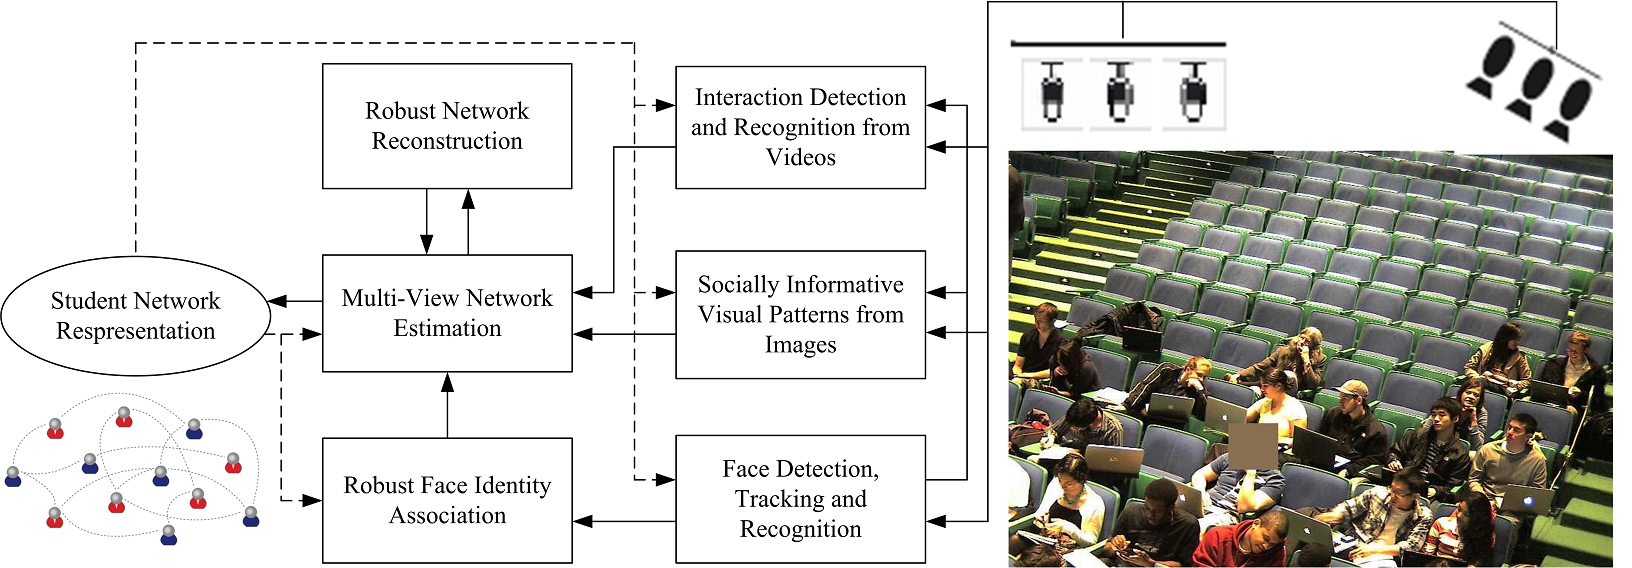
\includegraphics[width=\columnwidth]{prototype_1}
\end{center}
\vspace{-0.25in} \caption{\captionsize 
The prototype hardware and software infrastructure for analyzing socialized human behaviors in an indoor environment for social network estimation at Harvard University.\label{fig:prototype}\afterfigspace}
\end{figure}

The ultimate goal of our proposed research is a comprehensive system that seamlessly integrates a bottom-up hierarchy of multiple modules for sensing social networks from visual information. While an universally applicable framework or prototype system to accomplish this purpose is a long-term objective that may require more than affordable for the moment, at a reasonably constrained visual scene and a fixed group of social agents of small to medium scale is completely feasible and is on our agenda. We plan, for example, at a later stage of the award period, to move toward such a computer vision system that can reveal the heterogeneous and possibly time-varying social networks of all students that enroll in a semester-long course offered at Harvard University. 

As the initial attempt toward this goal to analyze socialized human behaviors in an indoor environment for social network estimation, we have built up a prototype hardware and software infrastructure at Harvard University. As shown in Fig. \ref{fig:prototype}, the hardware part of the prototype system mainly consists of a networked audio-visual recording system for large-scale recording of student interactions in a Harvard College lecture hall. The system records audio and video from approximately one hundred students during each lecture in conjunction with the audience responses through an online teaching-learning application. The video system uses six IP cameras that together provide resolution that is high enough to achieve face-based identity recognition of each student in the audience. The audio system is an innovative design consisting 48 omnidirectional boundary microphones mounted inconspicuously among the seats, and outputting sound from each microphone recording to a single user-friendly mp3 audio file.To automatically analyze the videos, we have developed a robust computational suite of computer vision tools. This software has consisted of several fundamental modules that detect, track, and recognize faces,  distill socially informative descriptions from raw images, and detect and recognize salient social interactions of interest, and has yielded the data used for our preliminary evaluation introduction in Section \ref{sec:activity}. The software suits, meanwhile, is expected to include other functionalities proposed in the previous sections by the end of the award period.

As illustrated by the diagram in Fig. \ref{fig:prototype}, and mentioned in the previous sections, we will employ the classroom observation system as our interface to harvest a volume of video sequences recording the indoor behaviors of the same class of students throughout the semester. The course that they enroll in uses interactive instruction by which they students are self-seated and engage in ad-hocly grouped discussions. We also maintain a teaching database where we have textual metadata regarding the students' profile data, status, learning performance, etc., as initial and partial social contexts among the students. This teaching database only only provides extra non-visual sources for estimating the student social network, but also can be used to provide the `ground-truth' networks to facilitate the research proposed in Section \ref{sec:vis2net}. Eventually, through the modules for face detection, tracking, recognition, and identify association (Section \ref{sec:assoc}), we link the members/nodes of the network to the human beings in each scene. Meanwhile, we detect socially meaningful interactions (Section \ref{subsec:activity}), co-occurrences, as well as compute other low-level visual cues for the purpose of estimating a `noisy' version of a multi-view network representation (Section \ref{sec:vis2net}), with the unobservable links between pairs in different views robustly reconstructed(Section \ref{sec:reconstruct}). The `hallucinated' social network from the videos in this way then provides the visually-sensed `honest' update for the network prior and is consolidated with the `textual' network as a comprehensive and more accurate characterization of this community. The feedback channel may infuse the updated social contexts and concepts to the face recognizer and the interaction detector. We expect such a close-loop socially-aware visual analytical framework to learn and self-build themselves in an evolving and unsupervised manner and to enable our new look at the images and videos in this socially networked era.


\subsubsection{Additional data acquisition and challenges}

Our proposed framework of social visual analytics is directly applicable to other `socialized imageries', such as online photo albums from Facebook or Flickr that we investigated in our previous work \cite{Stone2008,Stone2010}. We expect to employ a similar data acquisition model as introduced in \cite{Stone2008,Stone2010} for collecting complementing datasets from online sources.  In either the data from classroom interactions or materials harvested from online, there has been the challenges regarding privacy conservation and public availability of these materials. The way that we will adopt for prompting resource sharing and reproducible research will be in multiple levels. We will, for example, explore a way for `internal sharing', in which colleague researchers submit their companion prototype software and we evaluate it locally on their behalf. We will also seek to produce `privacy-conserved' version of the data, which can be a subset of the entire database with sensitive elements properly encrypted or removed. Finally and in particular, We will aim to provide new datasets that are free of privacy or publishability concerns, which serve for growing progress in the community with high potential and significant impact.









%With this established classroom observation system and these fundamental modules, we have successfully collected and processed a large-scale classroom behavior database consisting of 100 video clips in total. The students are seated in a regular lecture hall and are observed by a camera array with non-overlapping fields of view. The classroom is ``interactive'' because at various times throughout the lecture students are invited to engage in ad-hoc group discussions about problems provided by the instructor. The scale of our database is orders of magnitude larger than state-of-the-art computer vision datasets (e.g. those used in \cite{UTdata,Choi:context,Choi:recogtrack}), in the number of individuals (10-50 students per camera), the number of cameras (6), and the amount of time (100 minutes per camera, per recording, equaling over 3,000 minutes in total). Through a combination of face detection and tracking, we obtained noisy tracks for all students in each monocular video, upon which we developed descriptive modules that directly extract descriptiors such as head pose and body motion, we have also implemented a high-level module for behavior analysis based on similarity between two social groups, as depicted in Fig. \ref{fig:prototype}(b). In this module, the behavior of each individual is represented by a combination of the head pose and the motion of torso and arms (using the method of histogram of optical flows). The social behavior of a group is then represented by the configuration in space and time of the behaviors of its participants. With this social activity representation, the module detects a salient social activity from a new video and retrieves similar social activities from our established database. This functionality is illustrated in Fig. \ref{fig:prototype}(b), where our system has discovered a three-way conversation by identifying the participants of this conversation and the time span (several to tens of seconds) of this event. Based on the behavior representation for this space-time social interaction, the system searches the remainder of the database and retrieves a list of exemplars containing similar social behavior, ranked in the descending order of the similarities with the query. In this way, any manual annotations associated with the query video can be propagated to the top-ranking exemplars, and we are now taking this approach to propagate our manual annotations across the whole database. 








%At the current and initial stage of the effort to bring socialized semantics to computer vision, it can be usually the case that we do not have sufficient social contexts to help improving our target/face recognition, and we are not always specific about what are the meaningful social interactive activities that are most informative for social description. Conversely, we may neither know clearly about what exactly we should distill from images to fulfill a network learning task, nor have concrete knowledge about how the multiple views or overlapping community structures of a network will eventually turn out to be. However, we have argued at the beginning and demonstrated through the four proposed research problems the fact that the two aspects assist and benefit from each other, and an overall socially-aware visual analytical system is our ultimate goal. To this end, our final proposed research will include an attempt for a framework that eventually integrate social information and image understanding and allow them to learn and self-build themselves in an evolving and unsupervised manner.





